\chapter{Identify the Application Sector for your Analytic}

\subsubsection{Injuries prevention and return to play application}

This section will highlight and investigate one relevant application fields for BTS Bioengineering's gait pattern recognition analysis. An Italian motion analysis company that creates turn-key 3D Motion Capture, tri-axial Force Plate, Video and wireless \ac{emg}, hardware and software systems for research, clinical and sports. They offer quantifiable, objective data and follow the precise progress of each movement with their fully integrated systems, which measure the mechanics and dynamics of human motion.

\begin{figure}[h]
    \centering
    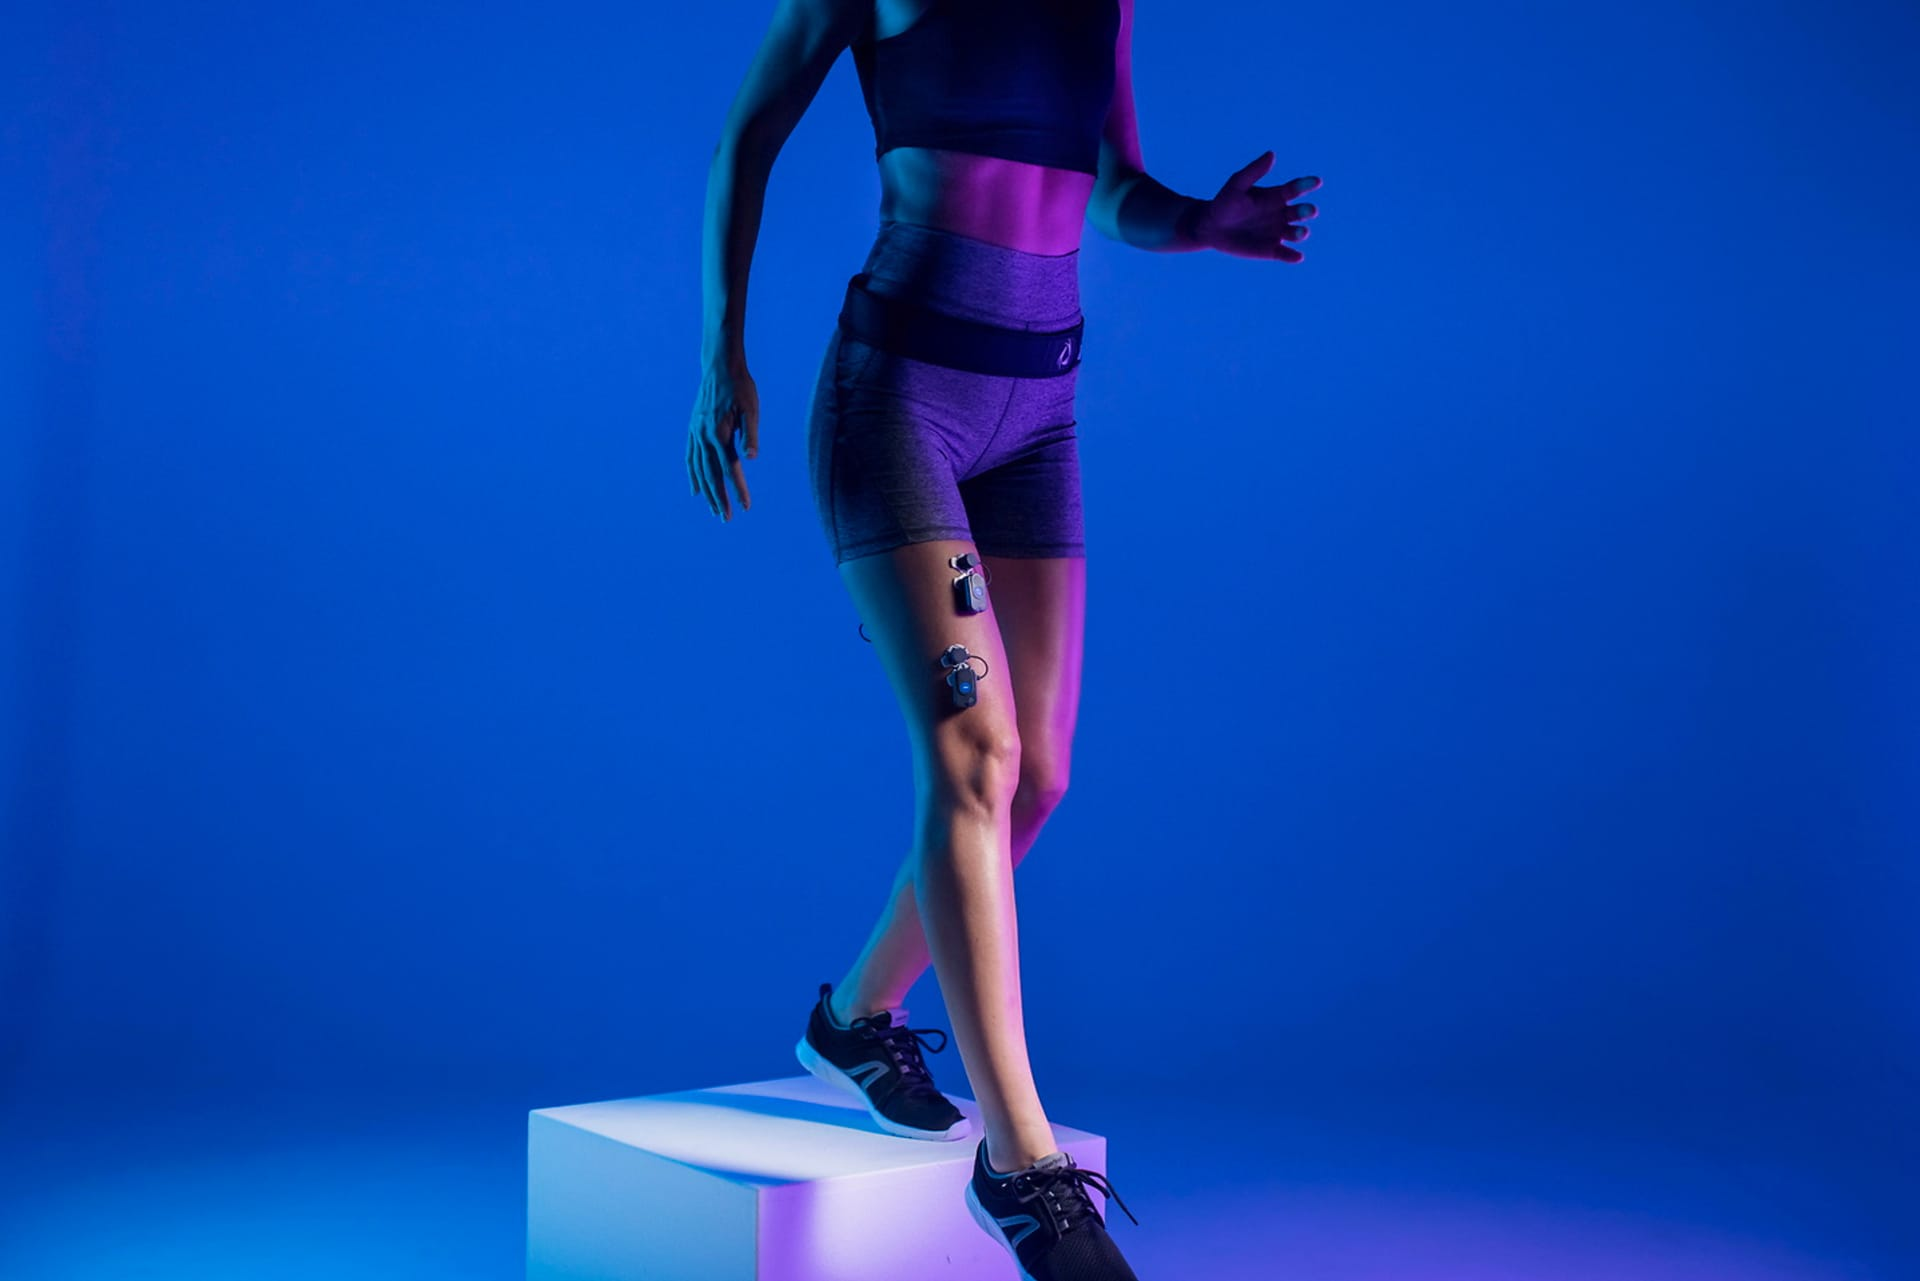
\includegraphics[scale=0.125]{Images/Injury prevention and return to play.jpeg}
    \captionsetup{justification=centering}
    \caption{Injury prevention and return to play \\ source: \cite{BTS_Injury_prevention2022}}
    \label{fig:Injury prevention and return to play}
\end{figure}


The primary goals of this application are injury prevention and the identification of optimal rehabilitation protocols in the event of injury \cite{BTS_Injury_prevention2022}. BTS Bioengineering's technologies and functional assessment tests are widely used by athletic trainers across several sports, for instance, MilanLab by AC Milan, PhysioeduLab, and Ripoll y de Prado Sport Clinic. Customers can keep track of the athlete's progress toward complete health by using the software's analysis techniques to monitor the athlete's progress and determine the optimal time for the athlete to return to playing competitive sports. As a result, the three primary features that stand out most about this application are the multiple-factor assessment service, the jump analysis, and the special protocols of particular sports movements.
